\documentclass[a4paper,oneside]{book}
\title{
\includegraphics[width=375px,height=100px]{Logo.jpg}}
\author{Marc-Christian Schulze}

\usepackage{listings}
\usepackage{color}
\usepackage{graphicx}
\usepackage{hyperref}
\usepackage[utf8]{inputenc}

\definecolor{dkgreen}{rgb}{0,0.6,0}
\definecolor{gray}{rgb}{0.5,0.5,0.5}
\definecolor{mauve}{rgb}{0.58,0,0.82}
\lstset{frame=tb,
  language=Java,
  aboveskip=3mm,
  belowskip=3mm,
  showstringspaces=false,
  columns=flexible,
  basicstyle={\small\ttfamily},
  numbers=left,
  numberstyle=\tiny\color{gray},
  keywordstyle=\color{blue},
  commentstyle=\color{dkgreen},
  stringstyle=\color{mauve},
  breaklines=true,
  breakatwhitespace=true,
  tabsize=2
}

\definecolor{blue}{rgb}{0,0,1}
\hypersetup{
    colorlinks, linkcolor={blue},
    citecolor={blue}, urlcolor={blue}
}

\begin{document}
\maketitle

\tableofcontents

\chapter{Introduction}
Mimicry is a non-intrusive network simulation framework for Java applications. Various other frameworks are currently available such as Tiny Sim, JNS, DSSim, Java Network Simulator, Peerfect and ns2. Typically these frameworks provide APIs which can be used to write prototype implementations of network protocols which then can be tested within a controlled environment. These kind of simulators typically provide a discrete behavior of the simulation. However, they are actually simulating prototypes.

The Mimicry framework does not require to compile the simulated applications to any part of the simulator's API. Instead it uses byte-code manipulation to load the application under test and intercepts all interactions with the JVM. This enables us to run the actual production ready code within the simulator.


\section{Download and Compile Mimicry}
Mimicry is currently only available via the Git repository so you need to download and compile the sources on your machine. In order to do so you first need to check that you've installed all prerequisites:
\begin{itemize}
\item JDK 7
\item Maven
\item Git
\end{itemize}
To check the latest source code out of git you need to run the following command in a shell:
\begin{verbatim}
git clone https://code.google.com/p/mimicry
\end{verbatim}
Now you can compile the Mimicry sources using Maven:
\begin{verbatim}
cd mimicry/parent
mvn clean install -DskipTests
\end{verbatim}
\textit{Note: You need to skip the unit tests since some of them are currently failing due to a bug.}
After the successful compilation a zip will be created in the target directory of the distribution project:
\begin{verbatim}
mimicry/mimicry-distribution/target
\end{verbatim}
Extract this archive to any location of your hard drive and make the \textit{mimicry.sh} shell script executable:
\begin{verbatim}
chmod +x mimicry.sh
\end{verbatim}


\section{Prepare an Application for Simulation}
In order to run your application Mimicry needs some information about where your binaries are located, how the classpath has to look like, how your main class is named, etc. This information is internally managed in a so-called \textit{ApplicationDescriptor}. Once you've setup such a descriptor Mimicry will be able to load and run your application.
In addition to the applications you also to setup the network itself, e.g. create nodes, define event stacks, etc. This is done in a Groovy-Script that is used to bootstrap and control the simulation.
A simple script for setting up a network with a single node and application could look like this:

\lstinputlisting{simple-script.groovy}

As you can see in the listing above the simulation setup consists of the following basic steps:
\begin{itemize}
\item Initialize the Network
\item Define EventStack and ApplicationDescriptors
\item Create Nodes and spawn Applications
\item Start the Timeline
\end{itemize}


\section{Run the first Simulation}
Mimicry ships with some predefined applications and simulation scripts. You can download them from
\begin{verbatim}
https://code.google.com/p/mimicry/downloads
\end{verbatim}
For illustration we'll use the PingPong-Example which runs two application instances sending each other messages using a TCP/IP connection.
After you've downloaded the \textit{example-PingPong.zip} you need to extract its content into the installation directory (where you did extract the compiled mimicry zip file).
Open a shell in that directory and run the following command:
\begin{verbatim}
./mimicry.sh pingpong.groovy
\end{verbatim}
This should bring up two console windows where in the first the server and in the second the client is writing its stdout to.


\chapter{Framework Architecture}
This chapter explains the architecture of the Mimicry framework showing how all the parts work together.

\section{Class Loading and Byte-Code Manipulation}
The core of the Mimicry framework is build by the internal used class loading mechanism in combination with byte-code manipulation at load-time. Using the custom class loading mechanism Mimicry isolates each simulated application from others and the actual framework. The byte-code manipulation is used to intercept all interactions of the simulated applications with the JVM. The application's byte-code is loaded in two phases:
\begin{enumerate}
\item Code Loading and Loop Interception

The actual class files are read from the hard drive using the Soot framework which transforms the byte-code into an intermediate representation that can be analyzed and modified. Leveraging the capabilities of Soot, loops are detected within the byte-code and a static method invocation added which is used for the life-cycle management later on. The resulting intermediate model is then transformed back to Java byte-code which is finally passed to the second phase.
\item Java API Interception

The second phase is realized using AspectJ to intercept the Java API. A specialized derivate of the \textit{WeavingURLClassLoader} is used to pass the modified byte-code to AspectJ which applies all aspects of Mimicry to the application's code.
\end{enumerate}
Both above-mentioned phases are implemented in a single class loader which is instantiated per simulated application instance. This isolates the instances from each other and allows to load classes multiple times (for each application) at the same time into the JVM. This approach is comparable to the one used in OSGi. The entire hierarchy of the class loaders used is depicted in Figure \ref{fig:ClassloaderHierarchy}.

\begin{figure}
\begin{center}
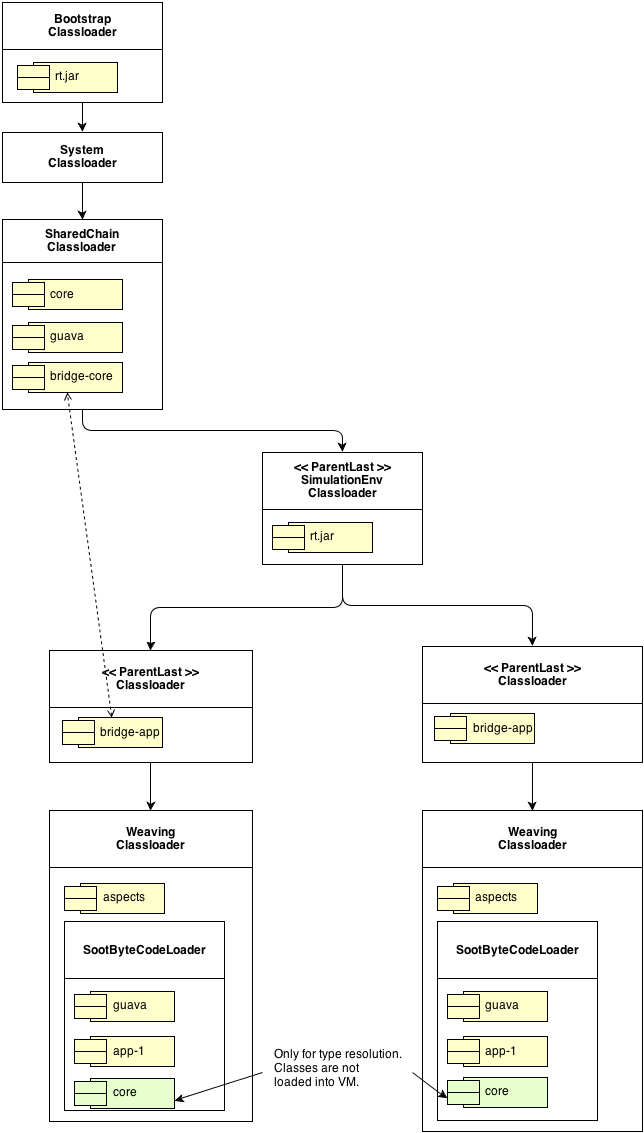
\includegraphics[width=\textwidth]{ClassloaderHierarchy.png}
\caption{The hierarchy of the ClassLoaders}
\label{fig:ClassloaderHierarchy}
\end{center}
\end{figure}

Each \textit{WeavingClassLoader} is responsibly for loading all application code and weaving it using Mimicry's aspects. On the next higher level a child-first or parent-last class loader is placed which prevents the \textit{WeavingClassLoader} from requesting application classes from the parent, which might also be able to load for instance the Guava library (since it's used internally). Those class loader instances are the actual border among the applications and the framework. A special package, called the Simulator Bridge, is located. This bridge is used by Mimicry's aspects to communicate with the simulation engine placed in the \textit{SharedChainClassLoader}.
Using the class loader of an application instance and reflection the \textit{SharedChainClassLoader} is able to access over the so-called Application Bridge the simulator bridge of each application individually.


\section{Event Processing}
The aspects woven into the simulated applications transform various API interactions into events which are then dispatched to Mimicry's event engine (cf. Figure ~\ref{fig:EventEngine}). This dispatching is done by the so-called \textit{Event Bridge} that furthermore manages all blocked control flows of the applications. The generated events are tagged with the application and control flow id and then passed to the underlying event stack. This stack can be configured per node in the simulation script. The event handler are responsible for implementing the actual simulation model you want to apply. Depending on the direction events are passed through the event stack they are called downstream or upstream events. An event handler is allowed to suppress events as well as generating new ones (even asynchronous). Event that reach the bottom of the event stack are dispatched to the event broker that notifies all other nodes as well as further listeners.
\begin{figure}
\begin{center}
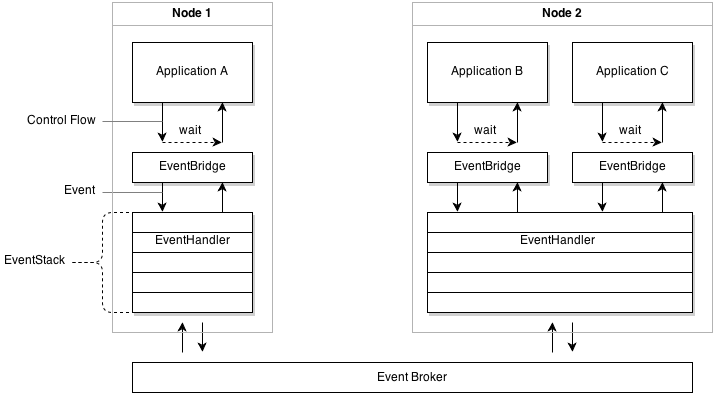
\includegraphics[width=\textwidth]{EventStack.png}
\caption{Architecture of the Event Engine}
\label{fig:EventEngine}
\end{center}
\end{figure}


\section{Application Lifecycle}
One important functionality of a simulator is to shutdown simulated application instances when desired. And indeed Mimicry is able to shutdown any application even if they run in infinite loops or are blocked due to synchronization. This is basically realized introducing aspects which cover thread instantiation, synchronization as well as loop interception. At the moment AspectJ is not capable of weaving loops but Harbulot and Gurd already proposed a possible extension in \cite{Harbulot:2006:JPL:1119655.1119666} and created a prototype implementation LoopsAJ (http://cnc.cs.man.ac.uk/projects/loopsaj/) which is based on top of abc (http://www.sable.mcgill.ca/abc/) and Soot (http://www.sable.mcgill.ca/soot/). 
However, using the soot framework Mimicry is already intercepting loop headers and checking each iteration whether the current managed thread is in shutdown phase. If so it throws a ThreadShouldTerminateException which is basically the same mechanism the JDK uses when \textit{Thread::destroy} is invoked. Furthermore the user code is prevented from catching this exception accidentally but intercepting all catch clauses and re-throwing that particular type of exception.
Finally, all timing related reason for blocking a control flow are handled with the actual clock implementation that works closely together with all threading aspects.


\section{Cluster Event Processing}
In order to allow Mimicry to scale to thousands of simulated nodes and applications the framework provides support for running Mimicry on a cluster of JVMs. This feature is currently not fully implemented but a preview can be seen in Figure \ref{clusterShowcase}.
\begin{figure}
\begin{center}
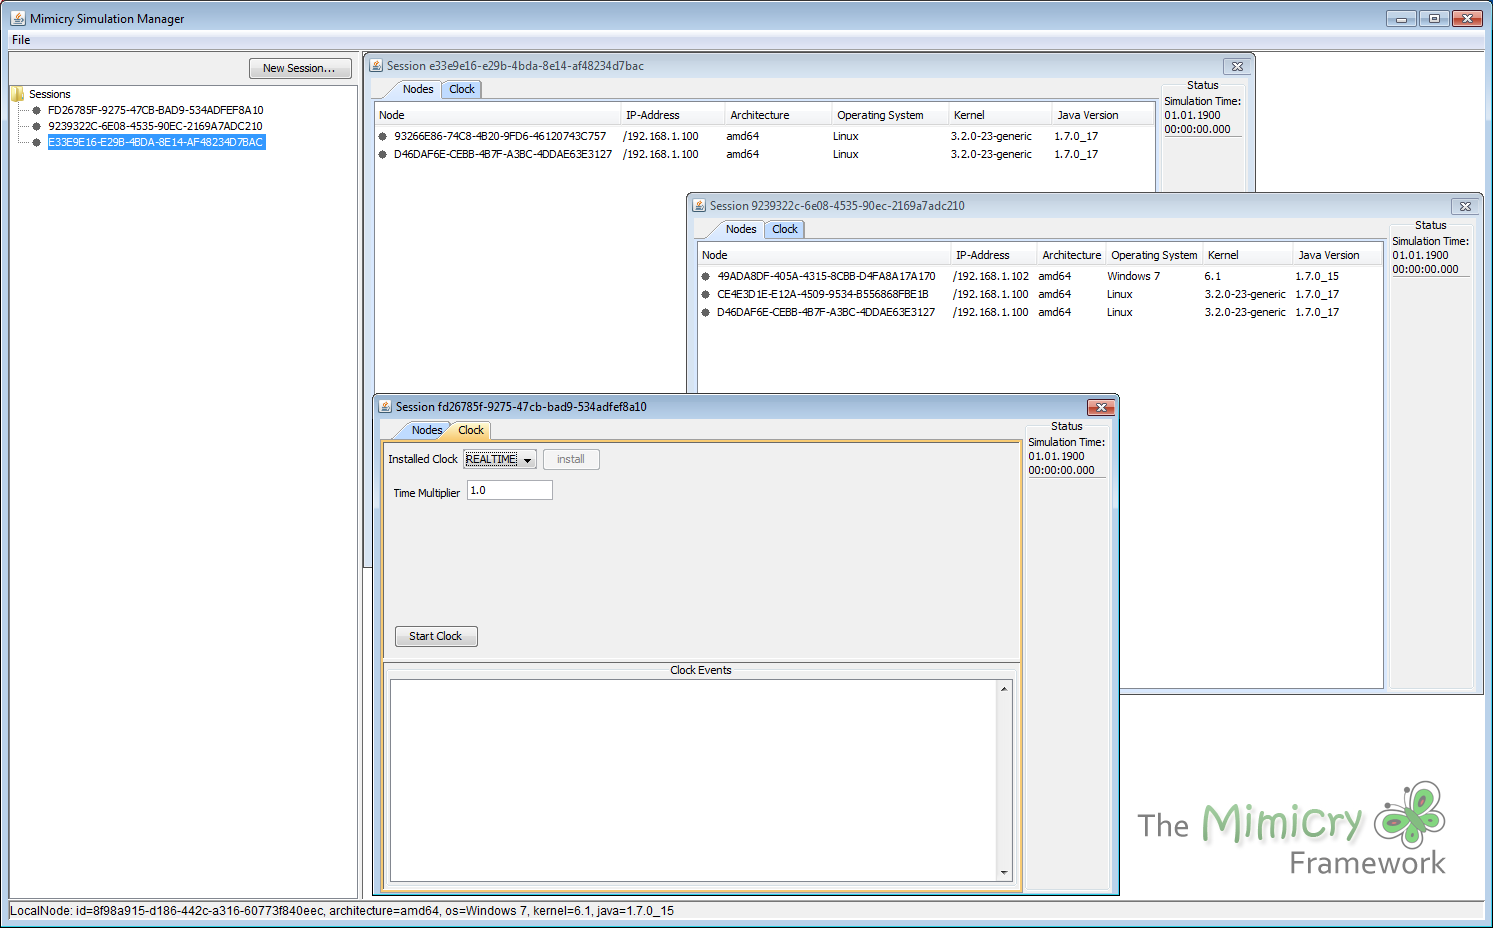
\includegraphics[width=\textwidth]{mimicry_showcase_03.png}
\caption{Preview of Mimicry's Cluster Support}
\label{clusterShowcase}
\end{center}
\end{figure}



\chapter{Extending the Mimicry Framework}
The Mimicry framework is meant to be extended by user simulations. A common case is to write custom event handler that implement special handling of TCP connection, e.g. simulation of bandwidth, jitter models, etc. Therefore this chapter shows how the most common extension points of Mimicry can be used. All extensions can be used without recompiling Mimicry itself. For this purpose several directories are used to create the framework's classpath:
\begin{itemize}
\item plugins/

This directory contains all event handler classes as well as dependencies of themselves. You can also refer to this code from within the simulation script.
\item lib/aspects/

Contains all compiled aspects that are applied to the application code. While this could be used to create new extension points within an application it's not recommended to do so without reading the existing aspects to avoid interferences.
\item lib/bridge

This directory contains all code that is loaded into the address space (class loader) of each application instance. This code is typically referenced by the aspects to generate events.
\item lib/shared/

Contains all classes shared between the bridge and the core framework. You would typically place your custom event classes within it.
\item lib/core/

This directory is not meant to contain custom user code.
\end{itemize}

\section{Event Handler}
The most common extensions are event handler that are necessary for each simulation. Therefore great care has been taken to create a simple but still powerful as well as robust API.
All event handler need to implement the interface \texttt{com.gc.mimicry.core.event.EventHandler} and must provide a publicly visible default constructor (since instantiation is done by Mimicry internally when required).
\lstinputlisting[firstline=18]{../../../../mimicry-core/src/main/java/com/gc/mimicry/engine/stack/EventHandler.java}
The two primary methods are handleUpstream and handleDownstream which are invoked by the event stack when events are passed up or down. You can also use a more abstract base class named \textit{EventHandlerBase}.
\lstinputlisting{../../../../mimicry-core/src/main/java/com/gc/mimicry/engine/stack/EventHandlerBase.java}
The use of the base class is recommended if you either are only processing upstream or downstream events; or you don't have to subclass anything else.
It's important to note that the event handler are entirely thread-safe as long as you don't spawn your own thread within. Instead use the given Scheduler instance which is synchronized with all other thread access to your handler instance. Furthermore you shouldn't create any UI elements such as frames or dialogs within your handler because it's not always the case that they are instantiated within your local JVM.
Sometimes you want to separate your handling code into different layers like in the ISO OSI model but still access the state of the other handler. Mimicry therefore has a built-in feature to obtain references to event handler within the same event stack. The \textit{EventHandlerContext} provides a method named \textit{findHandler} that takes a class and returns a proxy to the handler instance.
\begin{lstlisting}
MyHandler handler = getContext().findHandler(MyHandler.class);
\end{lstlisting}
The returned proxy can be safely invoked and the access is serialized on the thread responsible for the event handler. Note that obtaining the proxy is quite expensive and should therefore be done in the initialization method.
You can create proxies from interfaces which internally uses JDK's dynamic proxies as well as of classes which in that case uses CGLib.

Finally you might want to make your handler configurable by the simulation script. This can easily be achieved by implementing another interface called \textit{Configurable}.
\lstinputlisting[firstline=15]{../../../../mimicry-core/src/main/java/com/gc/mimicry/engine/stack/Configurable.java}
Once you've implemented that interface the framework will automatically inject the configuration provided in the simulation script into your event handler. The definition of the configuration might look like this:
\begin{lstlisting}
EventHandlerConfiguration[] eventStack = 
[
	[
		className: "org.example.MyHandler",
		configuration: 
		[
			key1: "value1",
			key2: "value2"
		]
	],
	...
]
\end{lstlisting}


\section{Event Listener}
Event listener allow you to write code that receives events without being part of any event stack. They can directly be registered at the \textit{EventBroker}. Unlike event handler they are not able to suppress events. They can only monitor the event stream and inject events asynchronously.
\lstinputlisting[firstline=11]{../../../../mimicry-core/src/main/java/com/gc/mimicry/engine/EventListener.java}
They are typically used to write plug-ins that are not located within an event stack but directly instantiated in the simulation script. An example of such a plug-in is the \textit{ConsoleWindowPlugin} that can be attached to an application in order to interaction with the command line of that particular instance.
\begin{lstlisting}
import com.gc.mimicry.plugin.ConsoleWindowPlugin;
// ...
ConsoleWindowPlugin.attach(network.getEventBroker(), appRef);
\end{lstlisting}

\section{Working with the Clock}
In the current implementation of mimicry the clocks of all application instances are in sync. This means it's currently not possible to set a different time for multiple nodes or applications. Nonetheless, the clock enables you to control the time line of all applications. The interface depicted in Listing \ref{lst:clockInterface} shows what can be done using the clock.
\lstinputlisting[caption={The Interface of a Clock}, label=lst:clockInterface,firstline=9]{../../../../mimicry-core/src/main/java/com/gc/mimicry/engine/timing/Clock.java}
Beneath offering the current time in milliseconds a clock provides 5 methods that are similar to the one provided by Java's base class \texttt{java.lang.Object} as well as one of \texttt{java.lang.Thread}. Those methods are basically the equivalent except that those having a timeout parameter also exist with an absolute time parameter. This is especially useful when we are working in multi-threaded environments where the delta time is specified by one but evaluated by another thread. An example can be found in the \texttt{ClockBasedScheduler}.
Using the clock the event handler are able to perform actions depending on the simulation time. For instance a TCP connection request could raise an error after the timeout specified in the \texttt{SO\_TIMEOUT} socket property has been elapsed.



\section{Custom Event Types}
All events must implement the \textit{Event} interface in order to processable by the event engine.
\lstinputlisting{../../../../mimicry-core/src/main/java/com/gc/mimicry/engine/event/Event.java}
In the current implementation the events don't make use of the VectorClock implemented in the Mimicry core which can later on be used to establish happened-before relations among recorded events.

\section{Built-In Event Types}
This section describes the existing event types and how they are raised and consumed by the application.

\subsection{Console Events}
The console of each application instance currently provides the following event types:
\begin{description}
\item[ConsoleInputEvent] \hfill \\
Can be emitted either by the simulation script or a plugin, e.g. the ConsoleWindowPlugin does exactly this when entering some text in the window.

\item[ConsoleOutputEvent] \hfill \\
Those events are emitted by the applications when it is writing something to stdout or stderr. Currently both streams are aggregated in the same event and no differentiation is possible.
\end{description}


\subsection{Networking Events}
The networking aspects currently provide the following event types:
\begin{description}
\item[SocketBindRequestEvent] \hfill \\
Is emitted by \textit{java.net.Socket}s that try to bind to a certain port. This event typically has a control flow associated that is blocked. You can respond to this event either with a SocketClosedEvent or a SocketBoundEvent.

\item[SocketClosedEvent] \hfill \\
Is either raised by the application when the \textit{java.net.Socket} has been closed or by an event handler when he decides to asynchronously close the socket. This event type does not require a control flow to be set. It's automatically picked up using the endpoint address.

\item[SocketConnectionRequest] \hfill \\
Raised by the application when a \textit{java.net.Socket} tries to connect to a certain address. You can either respond with a SocketClosedEvent or a ConnectionEstablishedEvent.

\item[ConnectionEstablishedEvent] \hfill \\
Raised by the event handler to indicate that a TCP/IP connection was successfully established.

\item[SetSocketOptionEvent] \hfill \\
Emitted by the application when a socket option has been changed.

\item[SetPerformancePreferencesEvent] \hfill \\
Raised by the application when the QoS parameters of the socket have been changed.

\item[TCPSendDataEvent] \hfill \\
Emitted by the application when someone writes something into the OutputStream associated with the socket.

\item[TCPReceivedDataEvent] \hfill \\
Emitted by the event handler to store data into the receive buffer of a TCP/IP socket which is picked up by the application using the socket's associated InputStream.

\item[SocketAwaitingConnectionEvent] \hfill \\
Emitted by a ServerSocket when its accept method is invoked by an application. Can be either responded to by a SocketClosedEvent or a ConnectionEstablishedEvent.

\item[SetDatagramSocketOptionEvent] \hfill \\
Emitted by DatagramSockets when the socket options are changed.

\item[SetMulticastSocketOptionEvent] \hfill \\
Emitted by MulticastSockets when the socket options are changed. Note that the common options with a DatagramSockets are indicated by a SetDatagramSocketOptionEvent.

\item[JoinMulticastGroupEvent] \hfill \\
Emitted by MulticastSockets if the joinGroup method is invoked.

\item[LeaveMulticastGroupEvent] \hfill \\
Emitted by MulticastSockets if the leaveGroup method is invoked.

\item[UDPPacketEvent] \hfill \\
Either emitted by a DatagramSocket, a MulticastSocket or an event handler.
\end{description}


\chapter{Using Mimicry}
This chapter shows the different ways on how to use Mimicry to run simulations.

\section{Standalone Setup}
coming soon...

\section{Cluster Setup}
coming soon...

\section{Unit-Test Setup}
coming soon...


\chapter{Built-In Extensions}
This chapter illustrates the usage of the built-in extensions of the Mimicry framework.

\section{EventHandler - PortManager}
The PortManager is an event handler that simulates the behavior of the operating system with respect to UDP and TCP port management. It keeps track of which application have bound a socket to a certain port and in which mode (exclusive or reusable). Furthermore it allows to query for this information using its public API. To detect which applications currently have sockets bound to a certain point you could obtain a handler proxy and read the current state.
\begin{lstlisting}
int somePort = ...;
PortManager portMgr = getContext().findHandler(PortManager.class);
Set<UUID> appIds = portMgr.getApplicationsOnPort(somePort);
\end{lstlisting}
This information is for instance used in the SimpleTCPDataTransport to determine to which application a certain TCP connection belongs.

\section{EventHandler - TCPConnectionManager}
coming soon...

\section{EventHandler - SimpleTCPDataTransport}
coming soon...

\section{EventHandler - SimpleUDPDataTransport}
coming soon...

\section{Plugin - ConsoleWindowPlugin}
coming soon... (cf. Figure \ref{ConsolePluginInAction})
\begin{figure}
\begin{center}
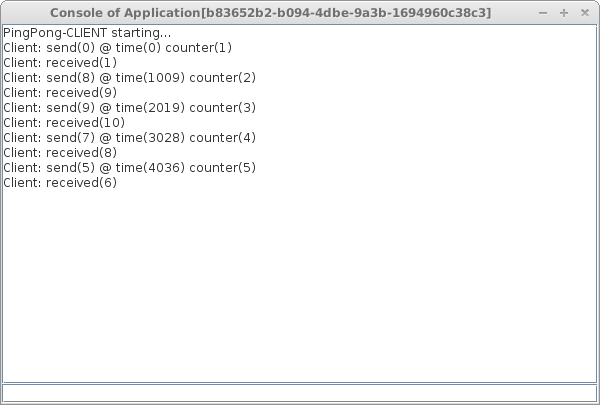
\includegraphics[width=\textwidth]{consolePlugin.png}
\caption{The Console Plugin in Action}
\label{ConsolePluginInAction}
\end{center}
\end{figure}

\section{Plugin - TimelineWindowPlugin}
This plugin allows you to control the timeline using a graphical user interface. (cf. Figure \ref{timelinePluginInAction})
\begin{figure}
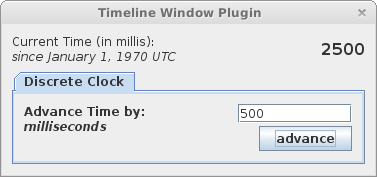
\includegraphics[width=0.5\textwidth]{timeline-Discrete.png}
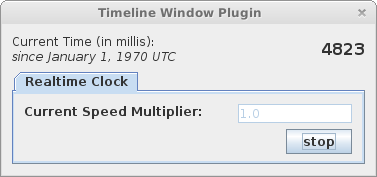
\includegraphics[width=0.5\textwidth]{timeline-Realtime.png}
\caption{The Timeline Plugin in Action}
\label{timelinePluginInAction}
\end{figure}


\chapter{Possible Extensions}
In this chapter some possible extensions to the Mimicry framework are documented which might be implemented in future releases.

\section{TCP/IP Connection Visualization}
Using the JUNG framework (http://jung.sourceforge.net/) it would be possible to display all TCP/IP connections in a directed cyclic graph using JUNG. This might be useful when debugging Peer-to-Peer applications such as Chord.

\section{JMX Proxy Generation}
It might be useful to implement a new aspect which automatically exposes Java objects after creation based on some filtering criteria. Using this feature the simulation script as well as other applications might be able to control the simulated applications in more detail.

\section{FileSystem Simulation}
Depending on the kind of simulated application it might be necessary to run them in a chrooted environment. Therefore intercepting all file system accesses would help in isolating.

\section{Checkpoints}
A *checkpoint* represents a certain state in the simulation where all threads are either
\begin{itemize}
	\item sleeping,
	\item waiting on a monitor,
	\item blocked by IO or
	\item in the front of a synchronized block.
\end{itemize}
Having checkpoints enabled you can
\begin{itemize}
	\item monitor the application's CPU utilization
	\item deterministically replay random numbers
\end{itemize}
But be aware that checkpoints decrease the application's performance.


\bibliographystyle{alpha}
\bibliography{Mimicry}

\end{document}
